\documentclass{article}
\usepackage{graphicx} % Required for inserting images
\usepackage[margin=2cm]{geometry} 
\usepackage{multicol,amsmath, amssymb}
\usepackage{xcolor}




\begin{document}
\begin{center}
    {\LARGE \textbf{Relations and Functions} }
\end{center}

\begin{multicols}{2}

  \subsection*{\textcolor{red}{Cartesian Products of Sets}}
The Cartesian product between two sets A and B is denoted by A × B is the set of all ordered pairs of elements from A and B

ie; $A \times B = \{(a, b): a \in A, b \in B\}$
\\
\textbf{Example: }consider the two sets $A= \{a_1, a_2\}$ and
$B = \{b_1, b_2, b_3, b_4\}$ \\
$A \times B = \{( a_1, b_1), (a_1, b_2), (a_1, b_3), (a_1, b_4), (a_2, b_1)\\
, (a_2, b_2),
(a_2, b_3), (a_2, b_4)\}.$
\\

\textbf{Properties: }
\begin{enumerate}
    \item Two ordered pairs are equal, if and only if the corresponding first elements
are equal and the second elements are also equal.
    \item   In general $A \times B \not = B \times A, \,but \, if\, A = B, A \times B = B \times A.$
    \item    n(A × B) = n(A) × n(B)
    \item n(A × B) = n(B × A)
    \item  If A and B are non-empty sets and either A or B is an infinite set, then so is
$A \times B$.
    $A \times A \times A = {(a, b, c) : a, b, c \in A}$. Here (a, b, c) is called an ordered
triplet.

   
\end{enumerate}


\subsection*{\textcolor{red}{Relations}}
A relation R from a non-empty set A to a non-empty set B is a subset of the Cartesian product A × B.

\textbf{Example:}Let  P = \{a, b, c\} and Q =\{ Ali, Bhanu, Binoy, Chandra, Divya\}. Then 

R = \{(a, Ali), (b, Bhanu), (b, Binoy), (c, Chandra)\} is a relation between sets P and Q

A visual representation of this relation R (called an arrow diagram) is shown in figure 

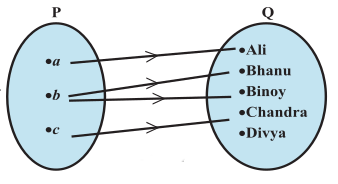
\includegraphics[scale=0.5]{1.png}

\begin{itemize}
    \item The second
element in the ordered pair is called the \textbf{image} of the first element
\item The set of all first elements of the ordered pairs in a relation R from a set
A to a set B is called the \textbf{domain} of the relation R.
\item The set of all second elements in a relation R from a set A to a set B is
called the \textbf{range} of the relation R. The whole set B is called the \textbf{codomain} of the
relation R. Note that range $\subset$ codomain.
\item The number of relation that can be written from A to B if n(A) = p, n(B) = q is $2^{pq}$.
\end{itemize}


A relation may be represented algebraically either by the \textbf{Roster
method} or by the \textbf{Set-builder method}.An \textbf{arrow diagram} is a visual representation of a relation.
  
\subsection*{\textcolor{red}{Functions}}
A relation f from A to B (f : A → B) is said to be a function if every element of set A has one and only one image in set B.

If f is a function from A to B and $(a, b) \in f$, then $f(a) = b$, where b is called the
\textbf{image} of a under f and a is called the \textbf{preimage} of b under b under f.

\begin{itemize}
    \item A function which has either R or one of its subsets as its range is called
a \textbf{real valued function}. Further, if its domain is also either R or a subset of R, it is
called a {real function}.
\end{itemize}

\subsection*{\textcolor{red}{Some functions and their graphs}}

\subsubsection*{Identity function}
 A function f : R → R defined by f(x) = x. Here the domain and range of f are R. The graph is a straight line  passing through the origin which makes 45 degrees with the positive direction of the x-axis.

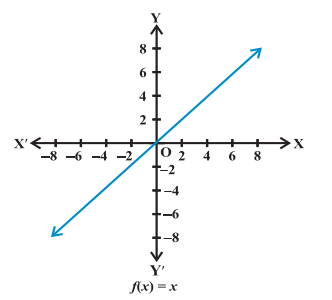
\includegraphics[scale=0.5]{2.png}


\subsubsection*{Constant function}
 A function $f : R \rightarrow R $ defined by $ f(x) = c$, where c is a constant.Here domain of f is R and its range is \{c\}.The graph is a straight line parallel to the x-axis.
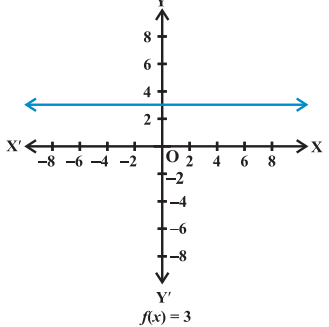
\includegraphics[scale=0.5]{3.png}

 \subsubsection*{Polynomial Function}
 A function f : R → R defined by
$f(x) = a_0 + a_1x + ….. + a_nx$, where n is a no-negative integer and $a_0, a_1, …., a_n \in R$

 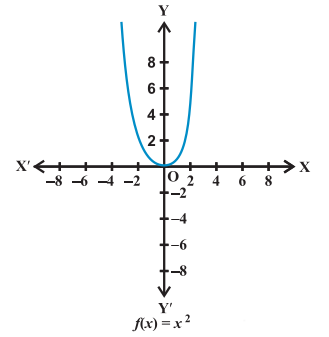
\includegraphics[scale=0.5]{4.png}
 
 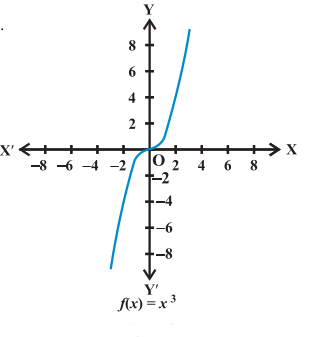
\includegraphics[scale=0.5]{5.png}

 \subsubsection*{Rational functions}
 A function $f: R \rightarrow R$ defined by $f(x)=\frac{p(x)}{q(x)}$, where $p(x), q(x)$ are functions of $x$ defined in a domain, where $q(x) \not = 0$

 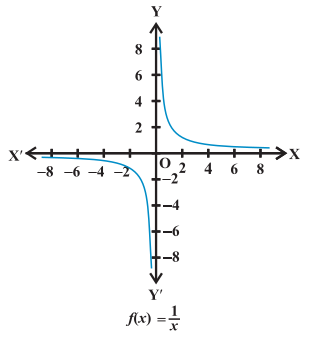
\includegraphics[scale=0.5]{6.png}


\subsubsection*{Modulus function}
 A function $f:R\rightarrow R$ defined by $f(x)=|x|$
 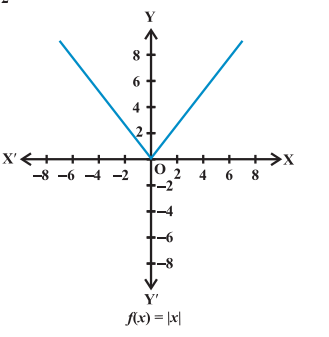
\includegraphics[scale=0.5]{7.png}

 \subsubsection*{Signum function}
 A function f: R → R defined by 
 \begin{equation*}
f(x)=
    \begin{cases}
        1 & \text{if } x>0\\
        0 & \text{if } x=0 \\
        -1 & \text{if } x >0
    \end{cases}
\end{equation*}
The domain of the signum function is R and the range is
the set \{–1, 0, 1\}

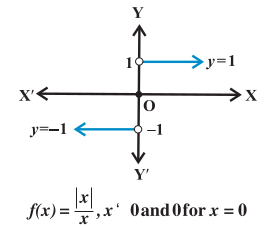
\includegraphics[scale=0.6]{8.png}

\subsubsection*{Greatest integer function}
f: R → R defined by 

 \begin{equation*}
f(x)=
    \begin{cases}
        \dots \\
        1 & \text{if } 1 \leq x < 2\\
        0 & \text{if } 1 \leq x < 1 \\
        -1 & \text{if } -1 \leq x < 0 \\
        \dots \\
    \end{cases}
\end{equation*}

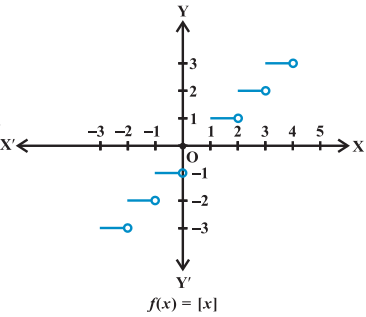
\includegraphics[scale=0.5]{9.png}


\subsection*{\textcolor{red}{Algebra of real functions}}
\begin{enumerate}
    \item \textbf{Addition of two real functions}:Let f : X → R and g : X → R be any two real functions, where $X \subset R$. Then, we define $(f + g) : X \rightarrow R$ by $(f + g)(x) = f(x) + g(x)$ for all $x \in X$

    \item \textbf{Substraction of two real functions}:Let f : X → R and g : X → R be any two real functions, where $X \subset R$. Then, we define $(f - g) : X \rightarrow R$ by $(f - g)(x) = f(x) - g(x)$ for all $x \in X$

    \item \textbf{Multiplication by a scalar}:Let f : X → R be a real-valued function and k be a scalar. Then, the product kf : X → R by (kf)(x) = kf (x) for all $x \in X$

    \item \textbf{Multiplication of two real functions}:Let f : X → R and g : X → R be any two real functions, where $X \subset R$ . Then, we define fg : X → R by fg(x) = f(x) × g(x) for all $x \in X$

    \item \textbf{Quotient of two real functions}: Let f and g be two real functions defined from
X→R, where $X \subset R$. The quotient of f by g denoted by
$\frac{f}{g}$ is a function defined by

$(\frac{f}{g})(x)=\frac{f(x)}{g(x)}$ Provided $g(x) \not = 0$ for $x \in X$

\end{enumerate}
 \end{multicols}
\end{document}
